\documentclass[xcolor={dvipsnames}]{beamer}

\usetheme{Malmoe}
\usecolortheme{seagull}
\usepackage[]{natbib}
\usepackage{textpos}
\usepackage{amsmath, amssymb, bm,mathtools}
\usepackage{multirow}
\usepackage{framed}
\usepackage{schemata}
\setbeamertemplate{navigation symbols}{}
\usepackage[english]{babel}
\usepackage{animate}
\usepackage{graphics}
\usepackage{fontawesome}


\definecolor{lightblue}{rgb}{0.145,0.6666,1} % Defines the color used for content box headers
\definecolor{Red}{rgb}{0.9,0.15,0}
\definecolor{Blue}{RGB}{55,126,184}
\definecolor{Green}{RGB}{77,175,74}
\definecolor{White}{RGB}{255,255,255}
\definecolor{Lightgray}{rgb}{0.86,0.86,0.86}


\setbeamertemplate{footline}
{
	\leavevmode%
	\hbox{%
		\begin{beamercolorbox}[wd=.50\paperwidth,ht=2.25ex,dp=1ex,center]{author in head/foot}%
			\usebeamerfont{author in head/foot}\insertshortauthor%% \beamer@ifempty{\insertshortinstitute}{}{(\insertshortinstitute)}
		\end{beamercolorbox}%
%		\hskip2pt%
		\begin{beamercolorbox}[wd=.50\paperwidth,ht=2.25ex,dp=1ex,center]{title in head/foot}%
			\usebeamerfont{title in head/foot}\insertshorttitle~~~~~~~~~~~~~~~~~~~~~~~~~~\insertframenumber
		\end{beamercolorbox}%
	}%
	\vskip0pt%
}
\makeatother

\title[Day 1]{
	\small{\textsl{}}\\$\,$\\$\,$}

\subtitle{\Large{\textsc{Decomposition techniques in population health research}}\\$\,$\\}


\author[European Doctoral School of Demography]
{
	\vspace{-0.5cm}
	\texorpdfstring{
		\begin{columns}
			\column{.9\linewidth}
			\centering
			\normalsize{Jos\'{e} Manuel Aburto}\\
			$\,$\\
			
\includegraphics[scale=0.12]{Figures/logos}     
		\end{columns}
	}
	{Jos\'{e} Manuel Aburto}
}

\date[]{}

\beamertemplatenavigationsymbolsempty
\begin{document}


\begin{frame}[plain]
	\titlepage
\end{frame}
%%%%%%%%%%%%%%%%%%%%%%%%%%%%%%%%%%%%%%%%%%%%%%%%%%%%%%%%%%%%%%%%%%%%%%%%%
%%%%%%%%%%%%%%%%%%%%%%%%%%%%%%%%%%%%%%%%%%%%%%%%%%%%%%%%%%%%%%%%%%%%%%%%%
\section{Outline}

%%%%%%%%%%%%%%%%%%%%%%%%%%%%%%%%%%%%%%%%%%%%%%%%%%%%%%%%%%%%%%%%%%%%%%%%%
\begin{frame}\frametitle{Preliminaries}
\Large{
		\begin{itemize}
		\item Introduction
		\item Course materials \url{github.com/jmaburto/EDSD-Decomposition-Course-2018}
		\item Assignment: 3 challenges in groups of 3 or 4.
		
		\end{itemize}
		
}

\end{frame}

\begin{frame}\frametitle{Outline}
\Large{
		\begin{itemize}
		\item The first decomposition method: Kitagawa (1955)
		\item Direct vs Compositional effects: Vaupel \& Canudas-Romo (2002)
		\item Change in life expectancy
		\end{itemize}
		
}

\end{frame}

\section{Kitagawa (2005)}

\begin{frame}\frametitle{Origins of decomposition}
\Large{
		\begin{itemize}		    
		\item Methods of standardization\\
		\hphantom{}
		\large{Aim: Eliminate compositional effect from overall rates of some phenomenon.}
		\pause
		\begin{itemize}
		\item Indirect standardization $\longrightarrow$ 1876
				\item Direct standardization $\longrightarrow$ 1844
		\end{itemize}
		\pause
				\hphantom{}
		\item \Large{Unreliable due to their dependence on an arbitrary standard}
		\end{itemize}				


}
\end{frame}


\begin{frame}
\begin{center}
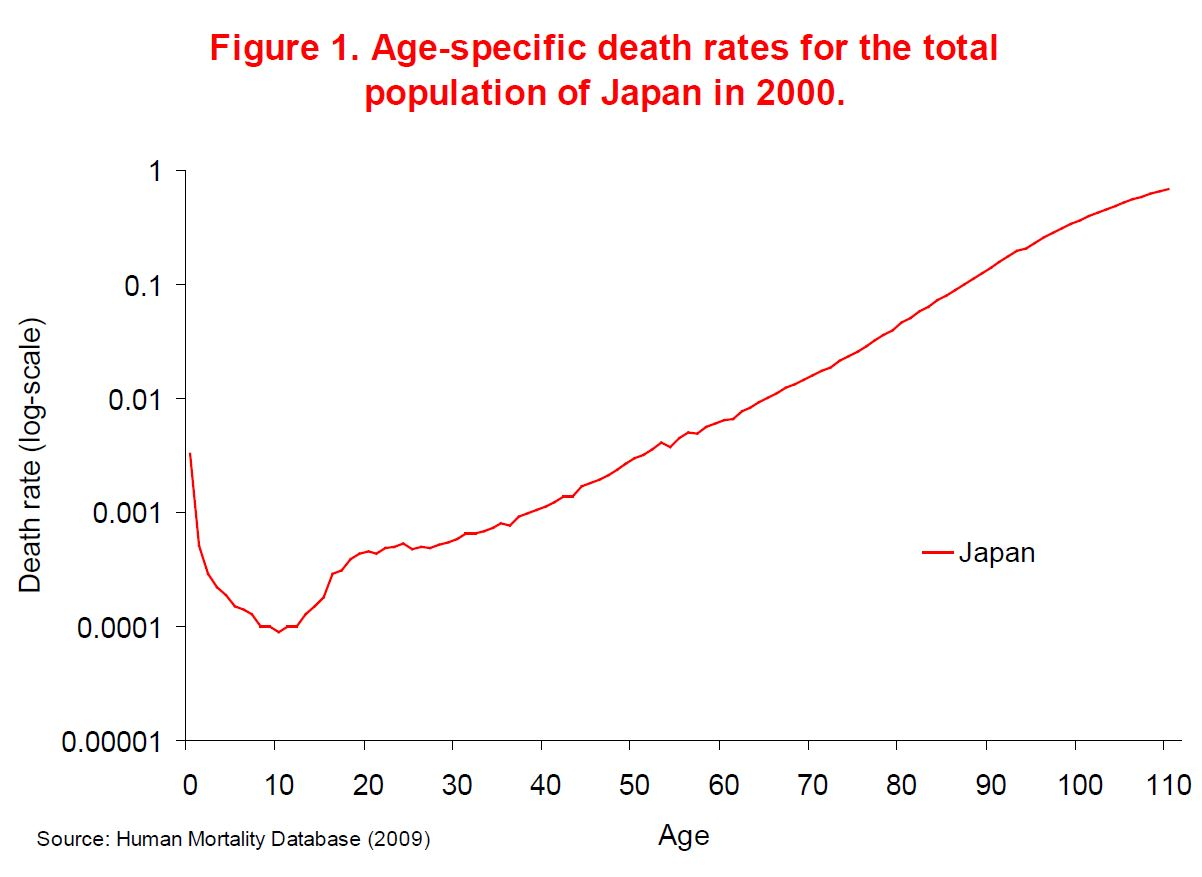
\includegraphics[scale=.3]{Figures/VCR1}
\end{center}
\end{frame}


\begin{frame}
\begin{center}
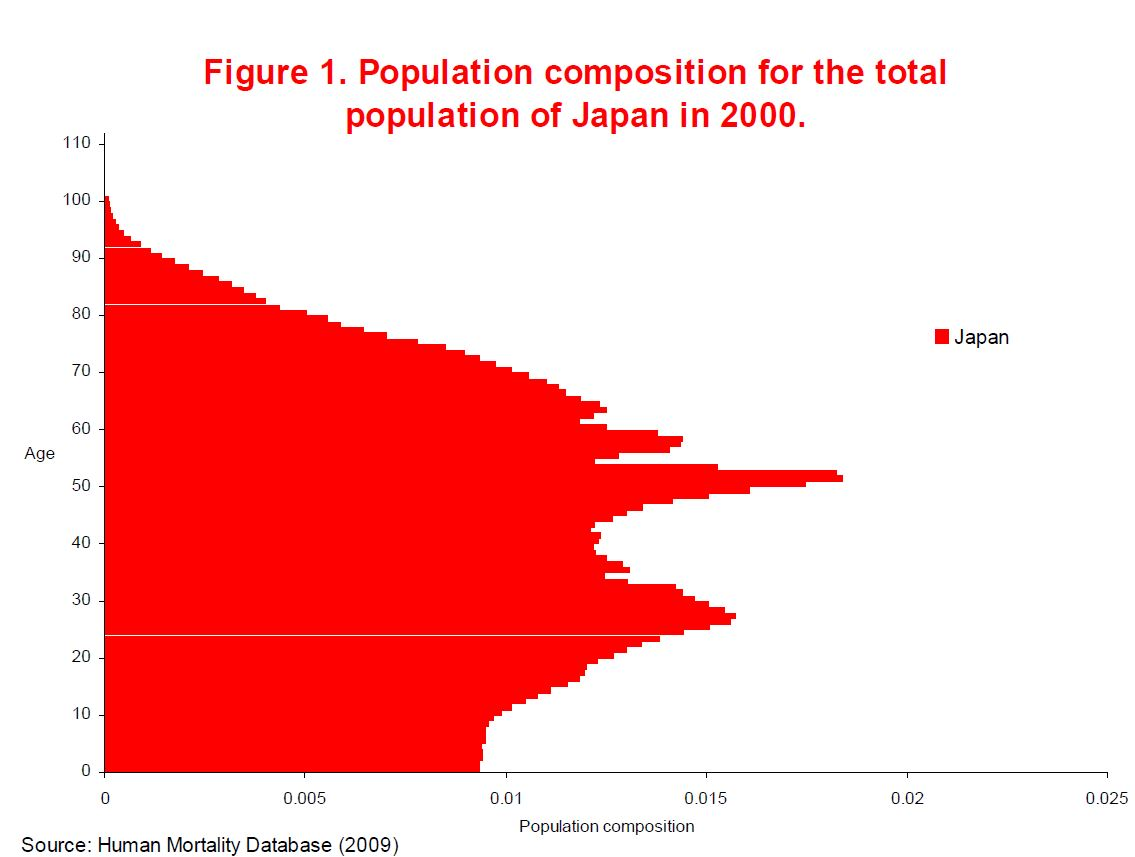
\includegraphics[scale=.3]{Figures/VCR2}
\end{center}
\end{frame}



\begin{frame}
\begin{center}
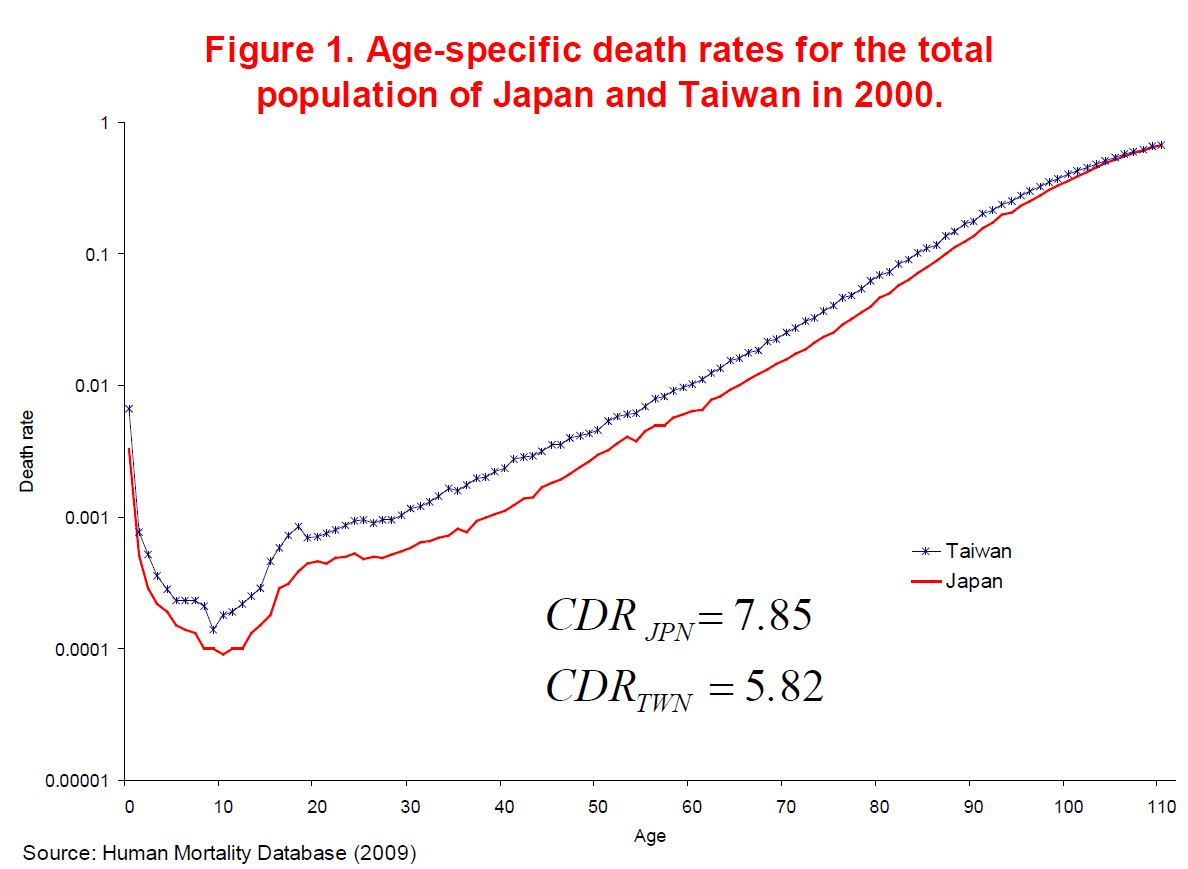
\includegraphics[scale=.3]{Figures/VCR3}
\end{center}
\end{frame}



\begin{frame}
\begin{center}
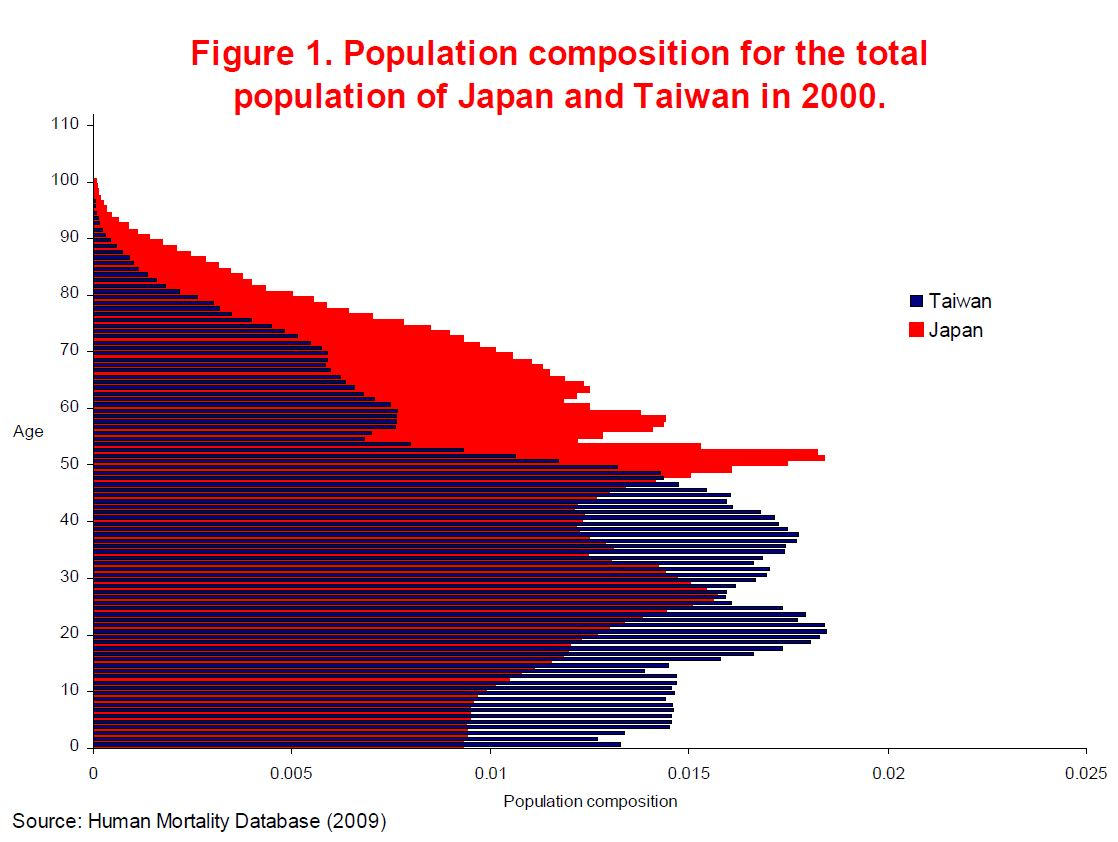
\includegraphics[scale=.3]{Figures/VCR4}
\end{center}
\end{frame}



\begin{frame}
\begin{center}
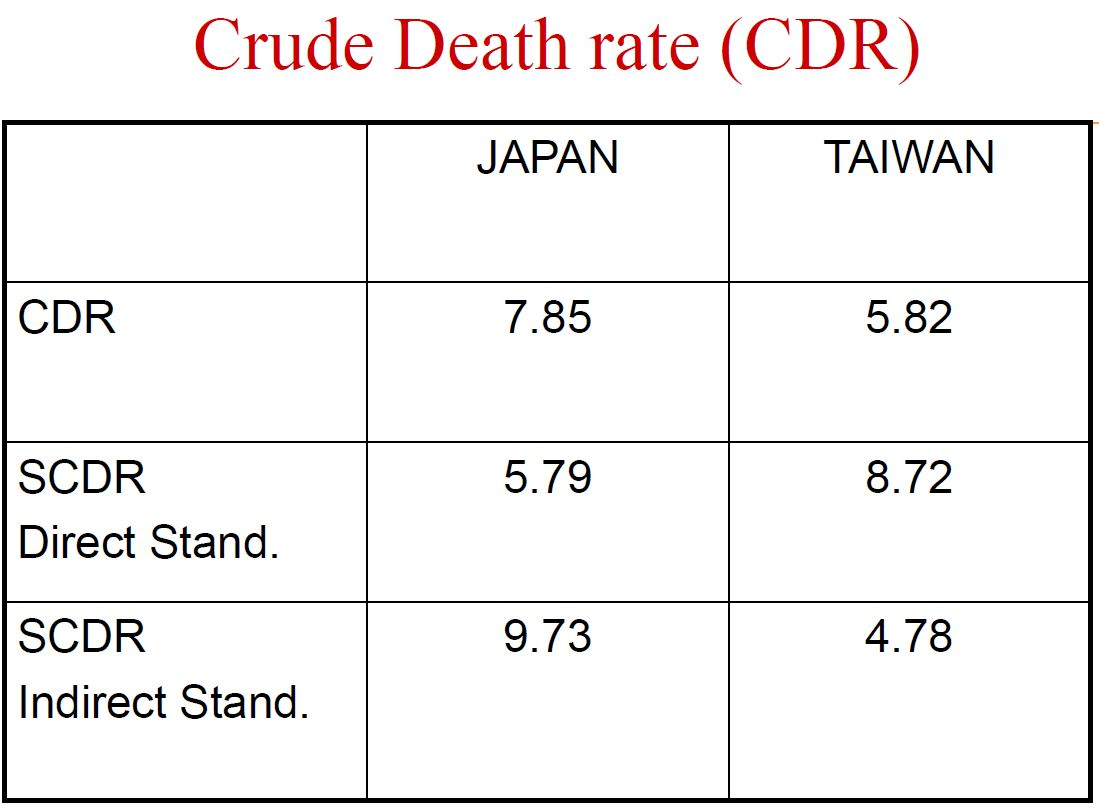
\includegraphics[scale=.3]{Figures/VCR5}
\end{center}
\end{frame}


\begin{frame}

\centering{\huge{Motivation to develop further methods of comparison: Decomposition}}


\end{frame}

\begin{frame}\frametitle{Kitagawa (1955)}
\large{
Notation for population 1 (population 2 same but lower cases):\\
		\hphantom{}
$N_i =$ number of persons in the i-th category of $I$\\
		\hphantom{}
$E_i =$ number of events (e.g. births, deaths) in the i-th category of $I$\\
		\hphantom{}
$T_i = E_i/N_i$ rate of persons in the i-th category of I\\
		\hphantom{}
$N = \sum_iN_i$ total number of persons\\
		\hphantom{}
$E = \sum_iE_i$ total number of events\\
		\hphantom{}
$T = E/N$ crude rate

}
\end{frame}


\begin{frame}\frametitle{Kitagawa (1955)}

The difference between the crude rates can be expressed as
		\hphantom{}
\begin{equation}
\label{eq.kitagawa}
\begin{split}
t-T  = &  \underbrace{\sum_iT_i\left[\frac{n_i}{n}-\frac{N_i}{N}\right]}_{\text{Changes in I-composition}} + \\
	& \underbrace{\sum_i\frac{N_i}{N}(t_i-T_i)}_{\text{Dif with pop 1 as standard}} + \\  
 	& \underbrace{\sum_i(t_i-T_i)\left[\frac{n_i}{n}-\frac{N_i}{N}\right]}_{\text{Interaction of rates and compositions}}
\end{split}
\end{equation}

\small{Optional exercise: show that $t-T$ can be expressed as \eqref{eq.kitagawa}}
\end{frame}

\begin{frame}\frametitle{Kitagawa (1955)}

To avoid the interaction term, Kitagawa suggests
		\hphantom{}
\begin{equation}
\label{eq.kitagawa2}
t-T  =  \underbrace{\sum_i \frac{t_i+T_i}{2} \left[\frac{n_i}{n}-\frac{N_i}{N}\right]}_{\text{Changes in I-composition}} +
\underbrace{\sum_i\frac{\frac{n_i}{n}+\frac{N_i}{N}}{2}(t_i-T_i)}_{\text{Changes in rates}}
\end{equation}

\small{Challenge 1: show that \eqref{eq.kitagawa} can be expressed as \eqref{eq.kitagawa2}}
\end{frame}


\begin{frame}\frametitle{Example: Berrington et al 2015}

Aim: To investigate the relative contributions of childlessness, timing, and quantum to educational differences in completed fertility within cohorts born between 1940 and 1969.\\
\hphantom{}
Data: General Household Survey (GHS) in Britain.
\hphantom{}

\end{frame}

\begin{frame}
Method: Completed family size ($C$) is equivalent to completed family size for mothers ($C_m$) times the proportion of women who are mothers ($p_m$) at the end of the reproductive period.For each 10-year birth cohort, we want to estimate the proportion of the total fertility differential between degree-educated (subscript H) and least-educated (subscript L) women that can be attributed to difference in childlessness.
\hphantom{}
\begin{equation*}
C_H-C_L=  \underbrace{\frac{p_{mH} + p_{mL}}{2}\color{blue}{(C_{mH}-C_{mL})}}_{\text{\Tiny{Cm weighted by avg. motherhood share}}}+
\underbrace{ \underbrace{\frac{ C_{mH}+C_{mL}}{2}(p_{mH} - p_{mL})}_{\text{\Tiny{Motherhood-share weighted by avg. completed fam size}}}}_{\text{Childlessness cotribution}}
\end{equation*}

\end{frame}

\begin{frame}
\[
\begin{aligned}
C_{mH}-C_{mL} = & \sum_i \left( \frac{\frac{N_{iH}}{N_H} + \frac{N_{iL}}{N_L}}{2} \right)(C_{mHi}-C_{mLi}) \\
& \sum_i \left(\frac{C_{mHi}+C_{mLi}}{2} \right)\left(\frac{N_{iH}}{N_H} - \frac{N_{iL}}{N_l} \right)  
\end{aligned}
\]

\pause

\small{
\begin{itemize}
\item  The second component reflects the extent to which Cm would change if age-specific fertility rates changed but the distribution of women at entry into motherhood remained constant.
\item The composition effect addresses the extent to which Cm would change if the distribution of age at entry into motherhood changed but the fertility rates conditional upon age at first birth remained constant.
\end{itemize}

}
\end{frame}





\begin{frame}
\begin{center}
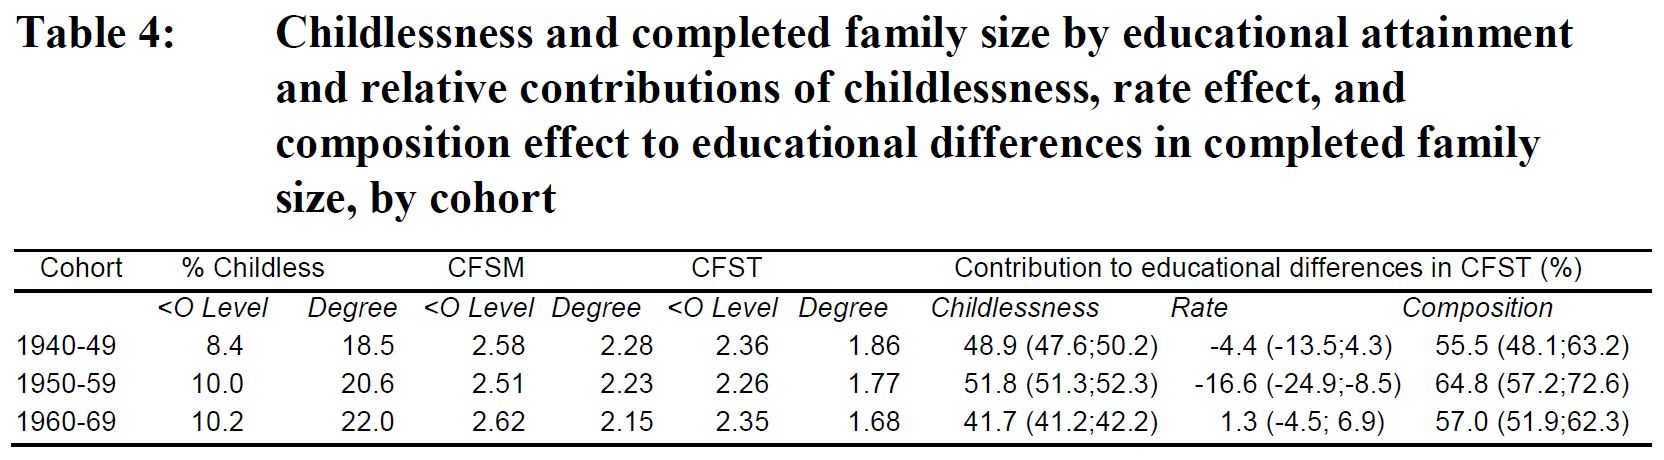
\includegraphics[scale=.25]{Figures/Berrington_results.JPG}
\end{center}

\end{frame}

\begin{frame}\frametitle{Further reading}
\begin{itemize}
\item Gupta, Prithwis Das. ``A general method of decomposing a difference between two rates into several components.'' Demography 15.1 (1978): 99-112.
\item Cho, L. J., \& Retherford, R. D. (1973). Comparative analysis of recent fertility trends in East Asia.
\item Gonalons-Pons, P., \& Schwartz, C. R. (2017). ``Trends in Economic Homogamy: Changes in Assortative Mating or the Division of Labor in Marriage?.'' Demography, 54(3), 985-1005.
\end{itemize}

\end{frame}

\section{Direct vs Compositional components}


\begin{frame}\frametitle{Direct vs Compositional}

\Large{Let $\bar{v}(y)$ denote the mean value of $v(x,y)$ over $x$ as
\hphantom{}
\begin{equation}
\begin{split}
E(v)=\bar{v}(y) & = \frac{\int_0^\infty v(x,y)w(x,y)dx}{\int_0^\infty w(x,y)dx}, \text{$x$ continuous} \\
		   & = \frac{\sum_x v(x,y)w(x,y)dx}{\sum_x w(x,y)dx} , \text{$x$ discrete}
\end{split}
\end{equation}
\hphantom{}

where $v(x,y)$ is some demographic function and $w(x,y)$ is some weighting function.

}
\end{frame}


\begin{frame}

\Large{A dot over a variable denotes the derivative with respect to $y$ (usually time)
\hphantom{}
\begin{equation*}
\dot{v}= \frac{\partial}{\partial y}v(x,y)
\end{equation*}
\hphantom{}

and an acute accent denotes the relative derivative or intensity with respect to $y$
\begin{equation*}
\acute{v}= \frac{\frac{\partial}{\partial y}v(x,y)}{v(x,y)} = \frac{\partial}{\partial y}\ln [v(x,y)]
\end{equation*}
\hphantom{}
}
\end{frame}


\begin{frame}
\centering{\huge{We want to decompose the derivative of $\bar{v}$ (e.g. mean age at childbearing, CDR) with respect to $y$ (time)} into \textcolor{blue}{direct} and \textcolor{red}{compositional} effects}
\end{frame}

\begin{frame}
\large{
\[
  \begin{aligned}
  \dot{\bar{v}} &= \frac{\partial}{\partial y} \frac{\int_0^\infty v(x,y)w(x,y)dx}{\int_0^\infty w(x,y)dx}\\ \pause
                &= \textcolor{blue}{\bar{\dot{v}}} + \textcolor{red}{\frac{\int_0^\infty v(x,y)\acute{w}(x,y)w(x,y)dx}{\int_0^\infty w(x,y)dx}} \\
                & \quad \textcolor{red}{ - \frac{\int_0^\infty v(x,y)w(x,y)dx}{\int_0^\infty w(x,y)dx}\frac{\int_0^\infty \acute{w}(x,y) w(x,y) dx}{\int_0^\infty w(x,y)dx}} \\ \pause
                &= \textcolor{blue}{\bar{\dot{v}}} + \textcolor{red}{E(v\acute{w})-E(v)E(\acute{w})} \\ \pause
                &= \textcolor{blue}{\bar{\dot{v}}} + \textcolor{red}{Cov(v,\acute{w})}
  \end{aligned}
\]
}
\end{frame}

\begin{frame}
\Large{

  \begin{equation}
  \dot{\bar{v}} = \textcolor{blue}{ \underbrace{\bar{\dot{v}}}_{\text{Direct component}} } + \textcolor{red}{ \underbrace{Cov(v,\acute{w})}_{\text{Structural or compositional component}}}
    \end{equation}

\pause
Main result in Vaupel \& Canudas-Romo (2002)
}
\end{frame}


\begin{frame}
\Large{
Open Exercise 1 in \texttt{R}
}
\end{frame}

\section{Change in life expectancy}

\begin{frame}
\Large{
Preliminaries:
\begin{equation*}
\mu(a), \text{force of mortality at age } a
\end{equation*}

\begin{equation*}
\ell(x) = \exp(-\int_0^x \mu(a)\, da), \text{survival function}
\end{equation*}

\begin{equation*}
e_o(a)=e(a,t)=\frac{\int_a^\infty\ell (a,t)\, da}{\ell (a)}, \text{life expectancy at age a}
\end{equation*}

\begin{equation*}
\rho = -\acute{\mu(a)}, \text{rate of mortality improvement}
\end{equation*}

}
\end{frame}


\begin{frame}
\Large{
\[
  \begin{aligned}
    \frac{\partial}{\partial t}\,e_o(t)=\dot{e}_o(t)	& = \int_0 ^\infty\frac{\partial}{\partial t}\,\ell(x,t)\,dx \\ \pause
    &=-\int_0^\infty\ell(x,t)\int_0^x\frac{\partial}{\partial t}\,\mu(a,t)\,da\,dx	\\ \pause
							& =-\int_0^\infty\frac{\partial}{\partial t}\,\mu(x,t)\int_x^\infty\ell(a,t)\,da\,dx\; \\ \pause
							&=\int_0^\infty \rho(x)e(x)f(x)dx
  \end{aligned}
\]

where $f(x)$ is the age-at-distribution weighting function.
}
\end{frame}


\begin{frame}
\begin{center}
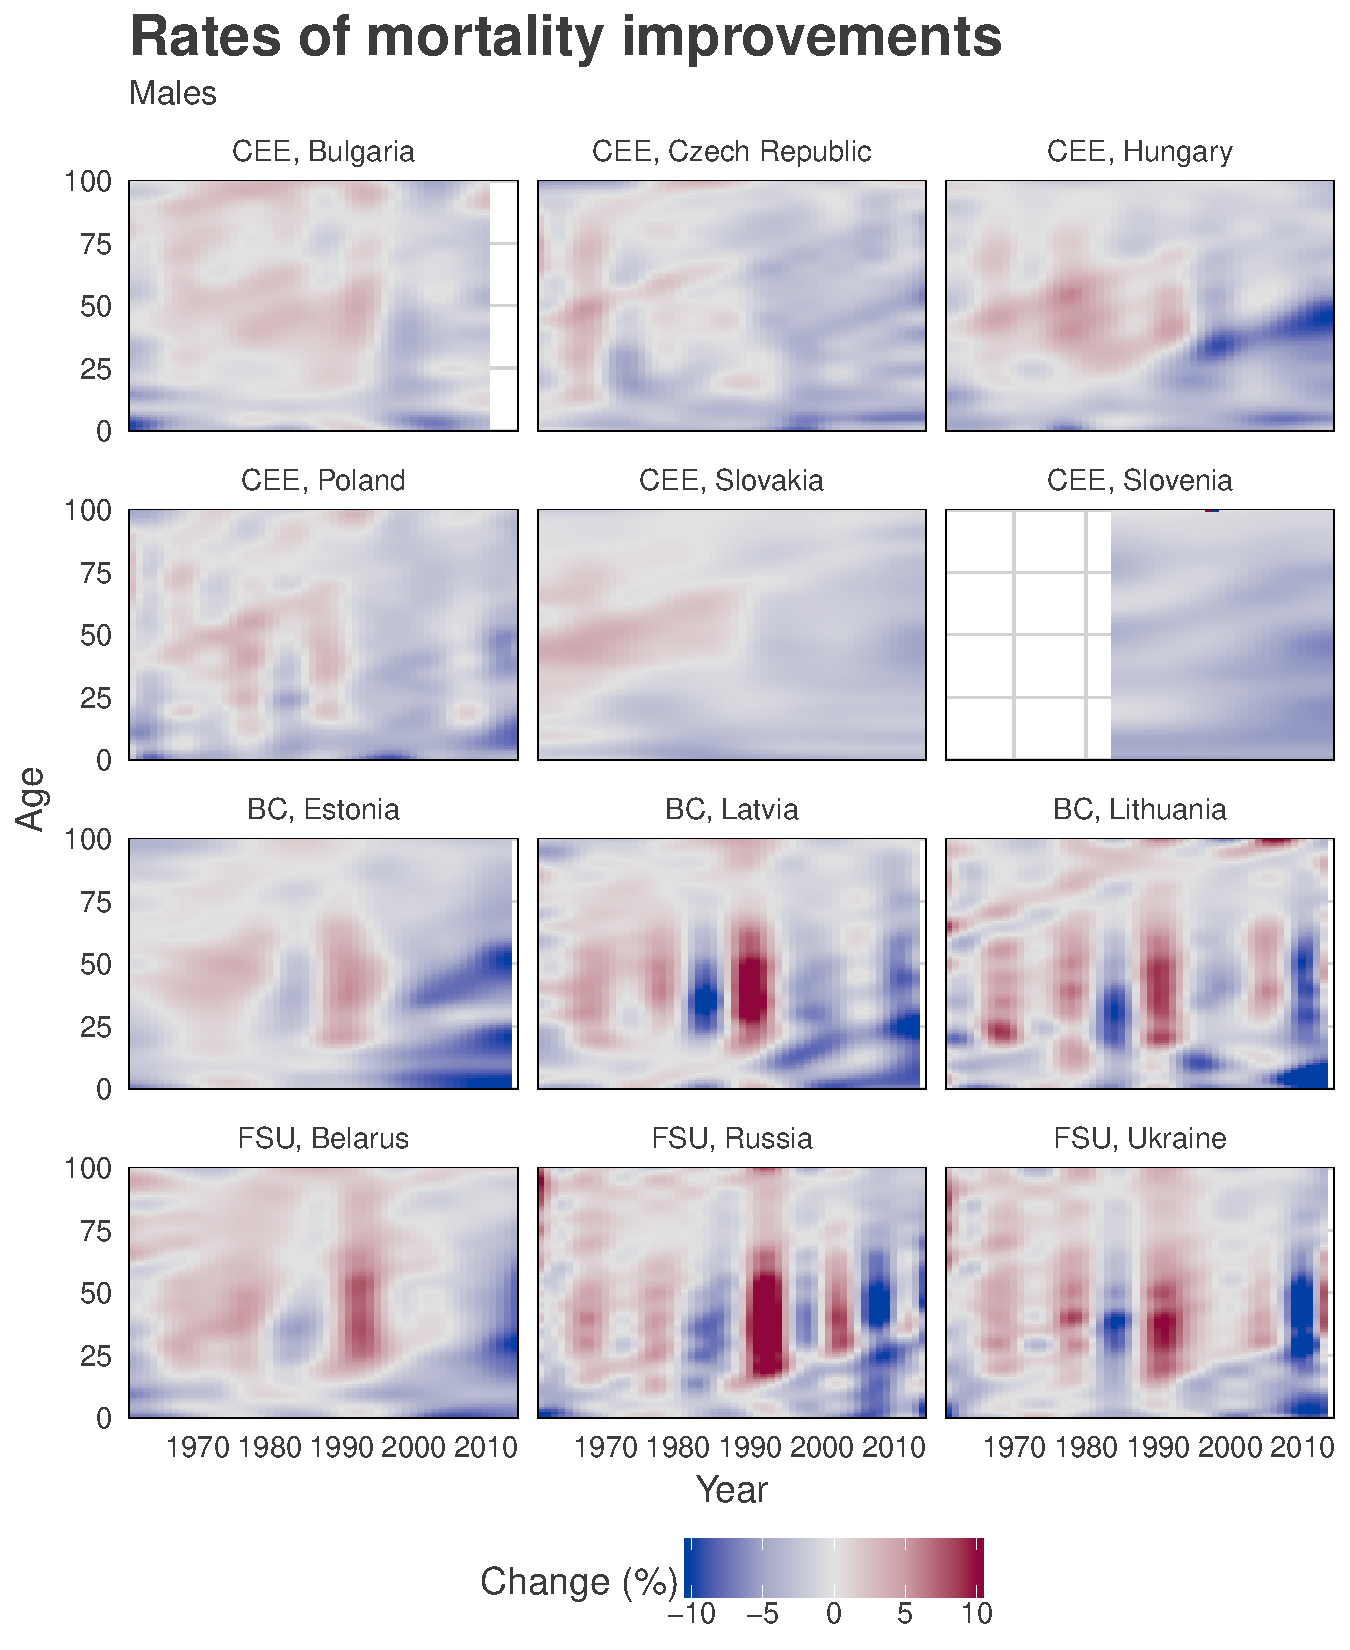
\includegraphics[scale=.28]{Figures/Romi_males}
\end{center}
\end{frame}


\begin{frame}
\begin{center}
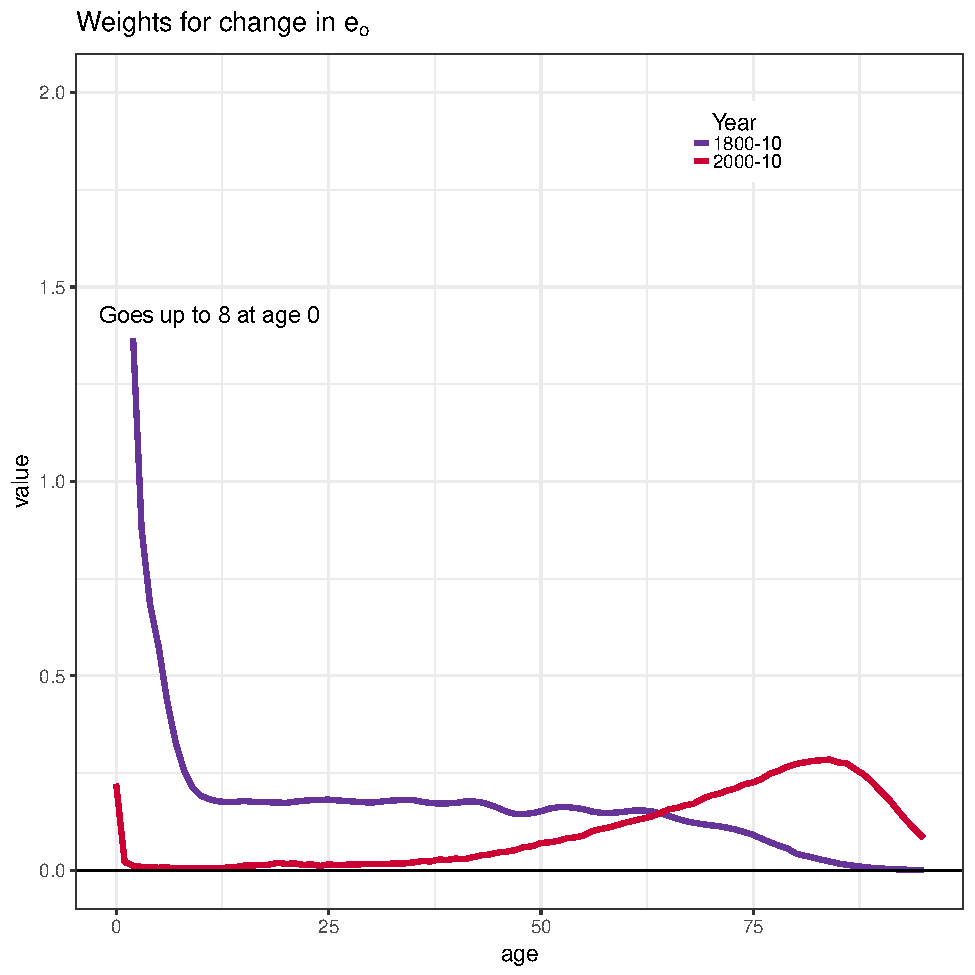
\includegraphics[scale=.5]{Figures/Sweden_weighs_e0}
\end{center}
\end{frame}


\begin{frame}
\begin{center}
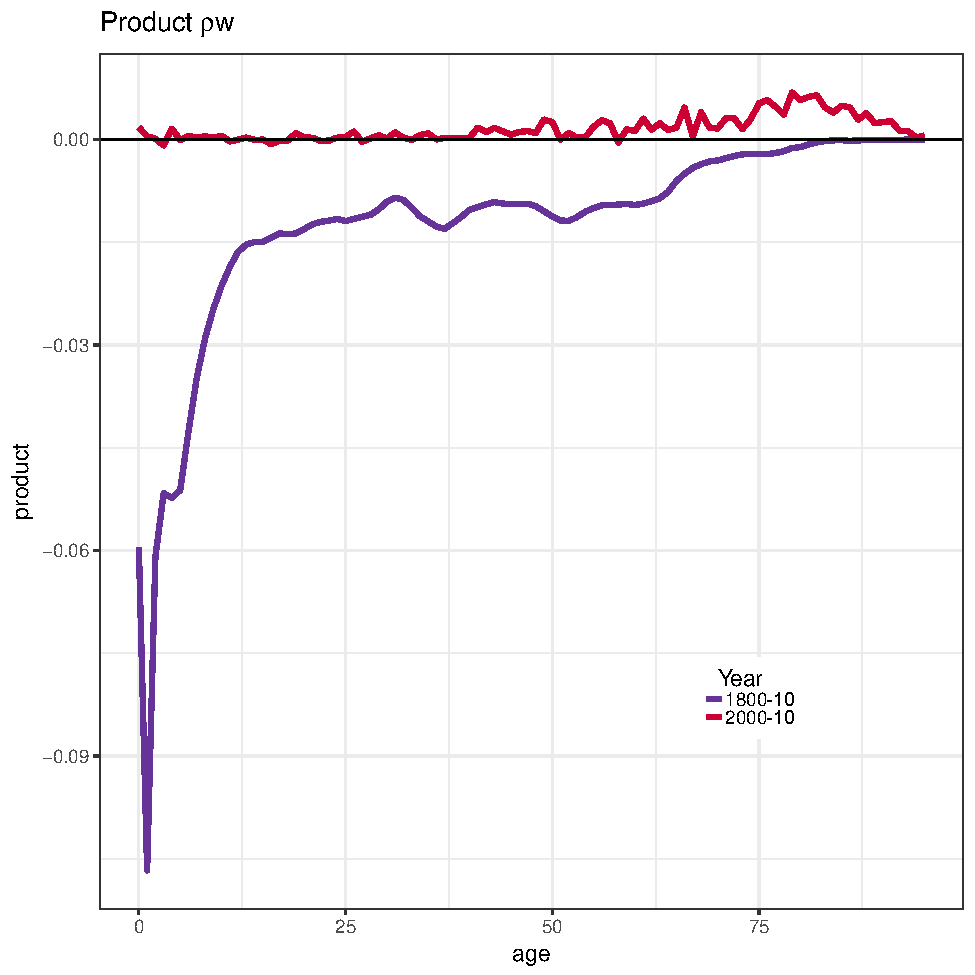
\includegraphics[scale=.5]{Figures/Sweden_product}
\end{center}
\end{frame}


\begin{frame}
\Large{Following Vaupel \& Canudas-Romo (2002)
\begin{equation}
\dot{e}_o(t) = \int_0^\infty \rho(x)e(x)f(x)dx
\end{equation}
can be written as:

\begin{equation}
\dot{e}_o(t) = \textcolor{red}{\bar{\rho}(t)}\textcolor{blue}{e^\dagger(t)} + Cov(\rho,e_x)
\end{equation}

where $\textcolor{blue}{e^\dagger=\int_0^\infty e(x)f(x)da}$ is the average life lost at time of death (Vaupel \& Canudas-Romo, 2003).

}
\end{frame}

\begin{frame}
\begin{center}
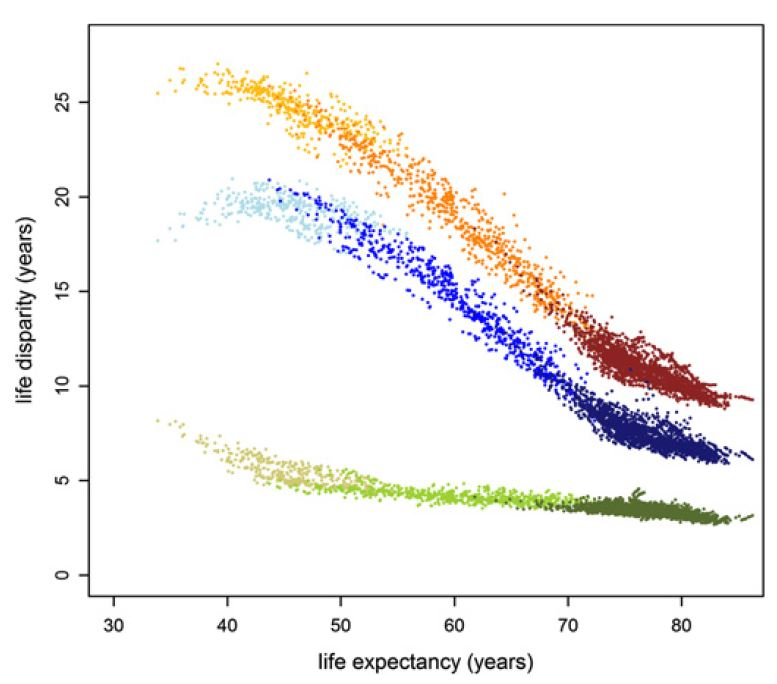
\includegraphics[scale=.39]{Figures/Life_disparity_1}
\end{center}

\tiny{Source: Vaupel et al 2011}
\end{frame}


\begin{frame}
\begin{center}
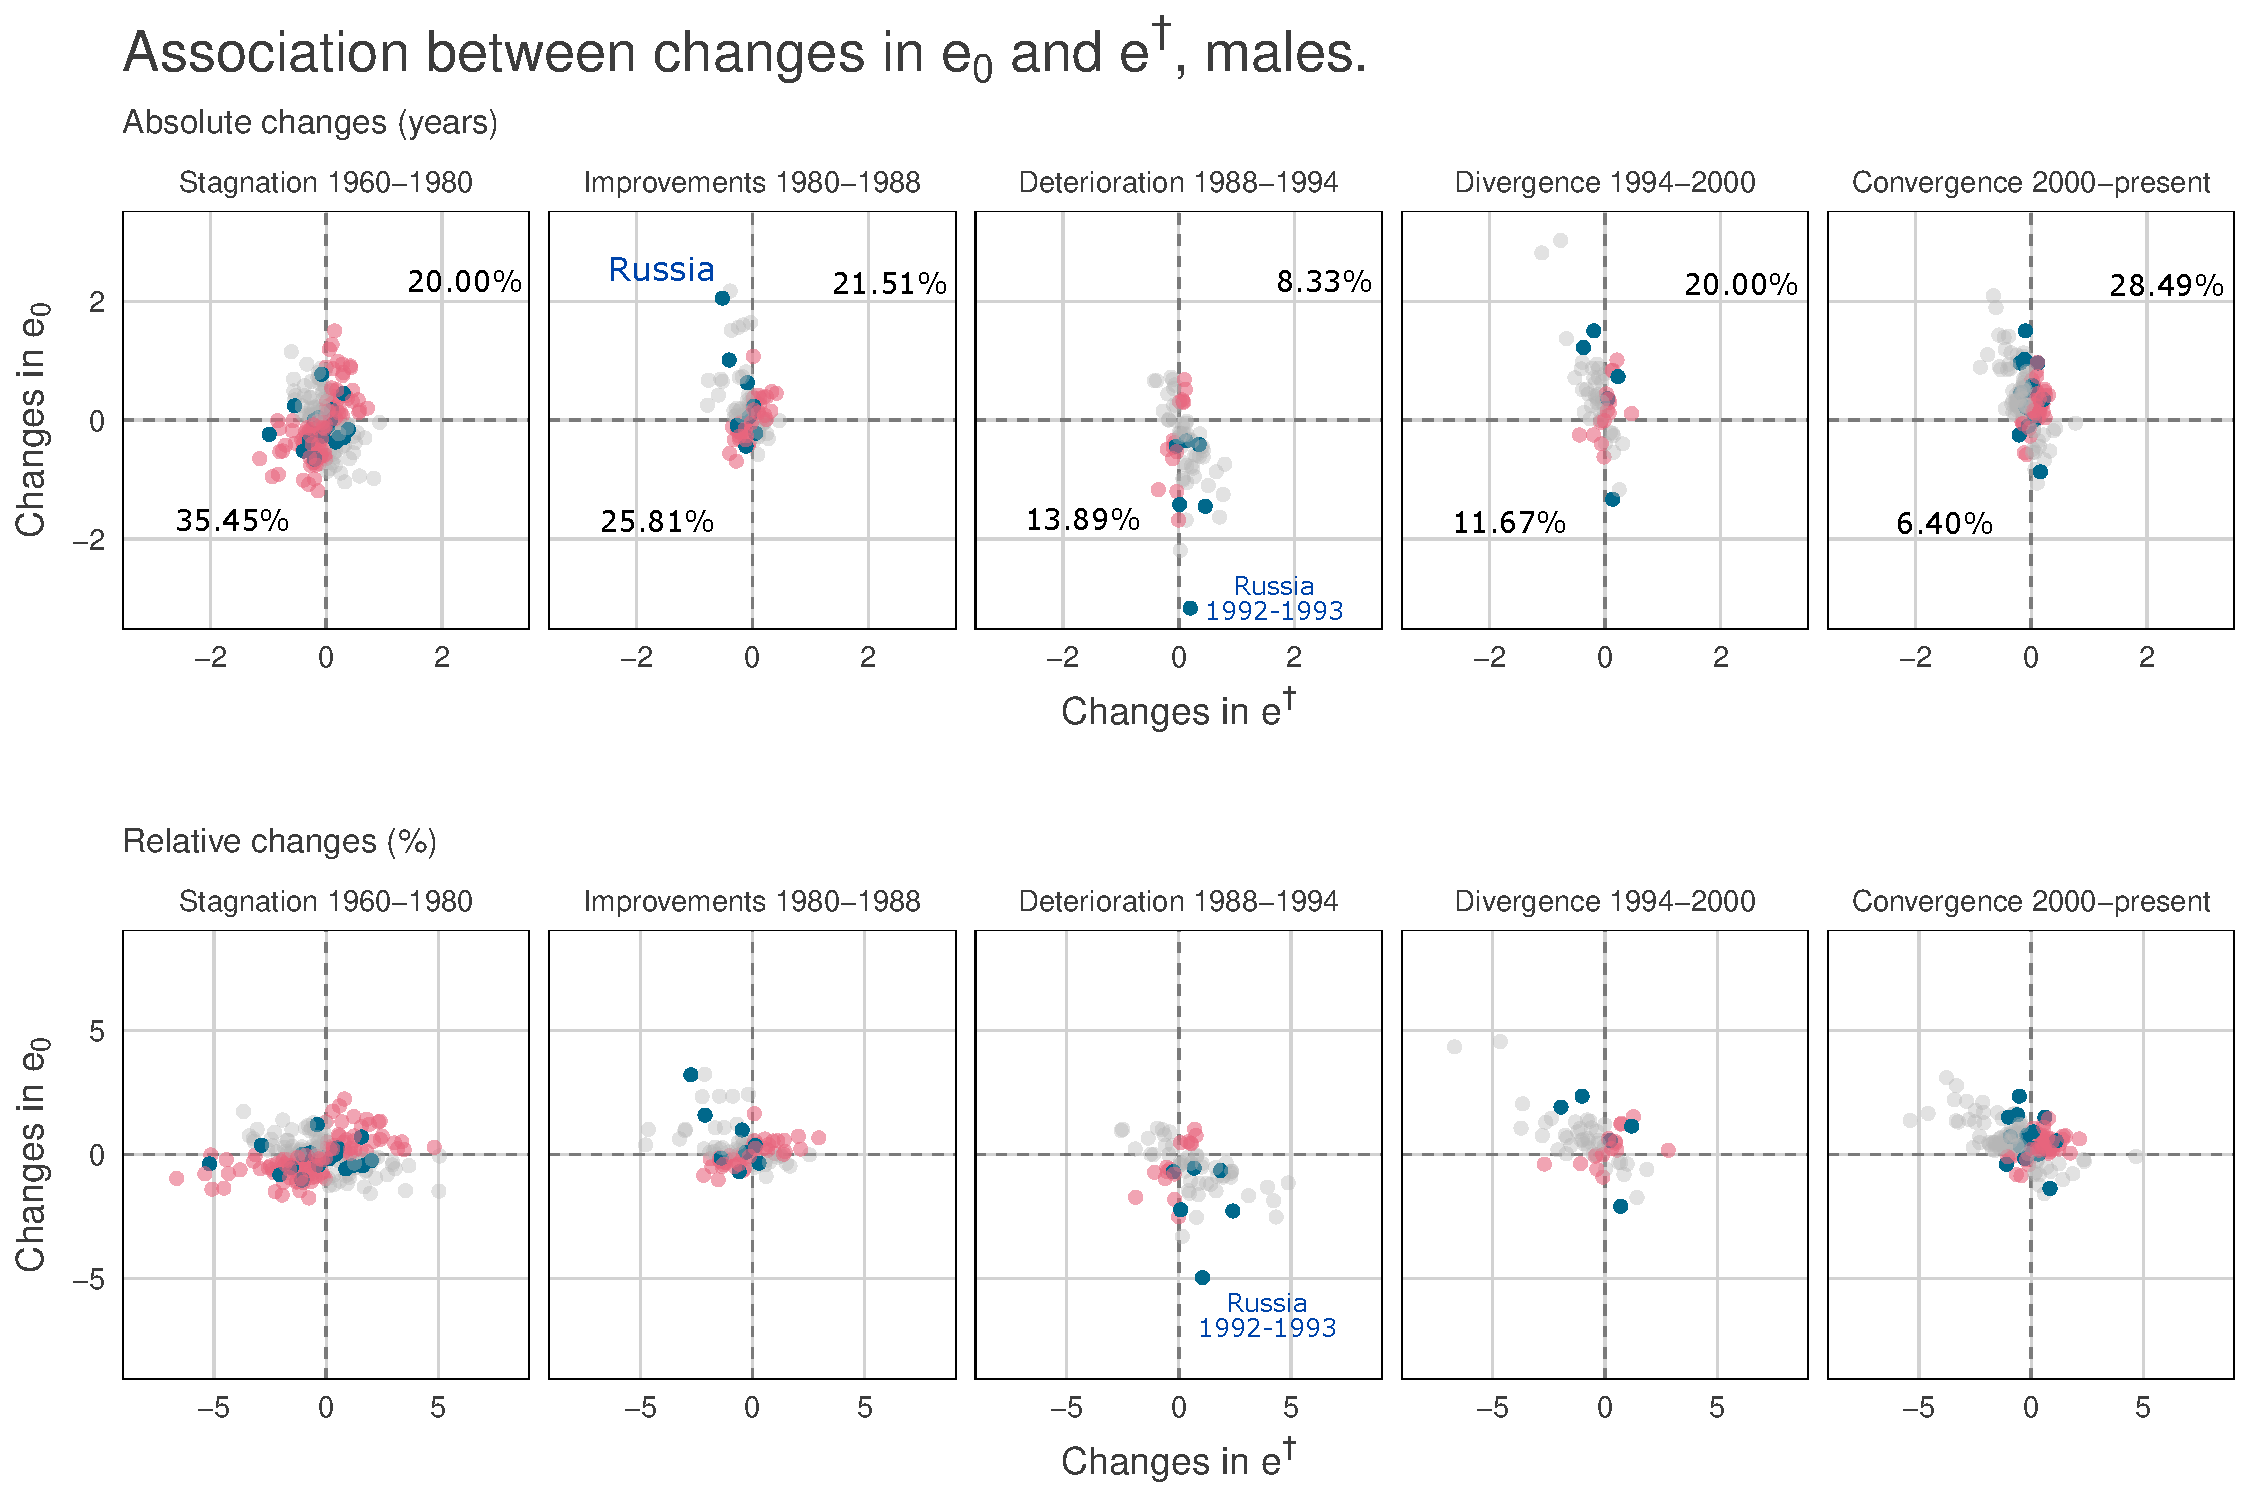
\includegraphics[scale=.28]{Figures/changes_males}
\end{center}

\tiny{Source: Aburto \& van Raalte 2018}
\end{frame}

\begin{frame}
\Large{Challenge 2: Using data from the UN give a descriptive (no more than 300 words with max 2 figures) answer to the question: Is there a female advantage in life disparity as there is in longevity? }
\end{frame}
\end{document}
	

